\begin{frame}
\frametitle{Introduction}
\centering
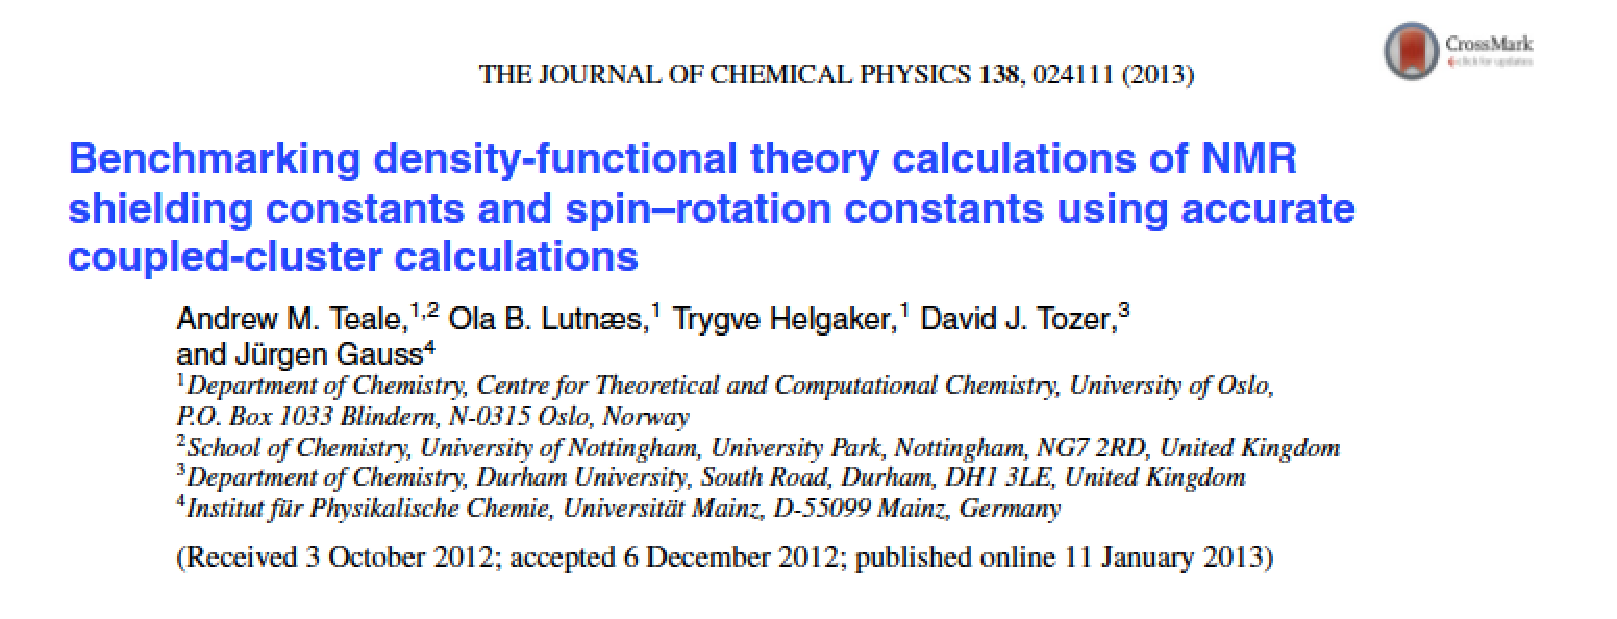
\includegraphics[scale=0.35]{figures/Teale_etal_2013.pdf}

\vspace{10mm}

\begin{columns}
\begin{column}[b]{0.5\textwidth}
    \textbf{Wave function methods}
    \begin{itemize}
        \item   RHF, CCSD, CCSD(T)
        \item   aug-cc-pCVXZ, X=D,T,Q
        \item   Basis set extrapolation
        \item   Comparison with experiment
    \end{itemize}
\end{column}
\begin{column}[b]{0.5\textwidth}
    \textbf{Density functional methods}
    \begin{itemize}
        \item   LDA, GGA, hybrid-GGA, OEP
        \item   aug-cc-pCVXZ, X=D,T,Q
        \item   Comparison with CCSD(T)
        \item   Comparison with experiment
    \end{itemize}
\end{column}
\end{columns}
\end{frame}
